% Two separate pairs: frozen-feature mechanism, then joint acquisition.
\newcommand{\SectionSpectrumFigure}{%
\begin{figure}[!htbp]
 \centering
 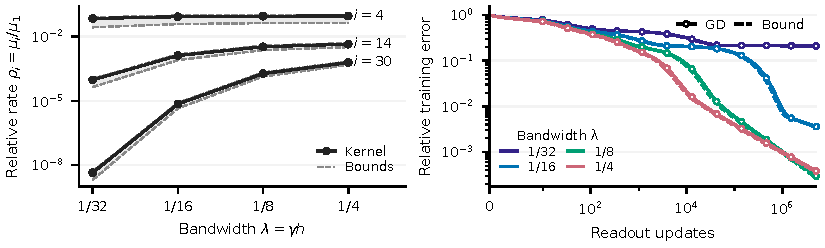
\includegraphics[width=\linewidth]{output/diagnostics/section34_long_horizon/main_5m/paired/spectrum_readout.pdf}
 \caption{\textbf{Small slopes weaken kernel directions and delay readout learning.}
 \textbf{A:} finite-kernel ratios (dots) and theorem intervals (dashed
 boundaries, shading) at four bandwidths. Lines connect ordered ranks;
 eigenvectors change with bandwidth. \textbf{B:} executed frozen-GD relative
 output errors (solid) and square roots of the theorem's lower bounds
 (dashed), through five million updates. Both panels use width~512 and the
 same target and geometry (Appendix~\ref{app:note-evaluation}).}
 \label{fig:note-spectrum}
\end{figure}
}

\newcommand{\SectionTrainingFigure}{%
\begin{figure}[!htbp]
 \centering
 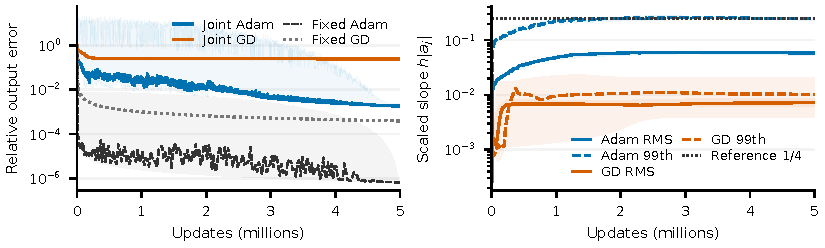
\includegraphics[width=\linewidth]{output/diagnostics/section34_long_horizon/main_5m/paired/joint_acquisition.pdf}
 \caption{\textbf{Partial slope acquisition leaves a precision gap.}
 \textbf{A:} joint Adam/GD relative output errors and frozen uniform
 $\lambda=1/4$ references under the same five-million-update budget.
 \textbf{B:} RMS and 99th-percentile scaled slopes $h|a_j|$ in A's joint
 runs. The reference is a supplied geometry, not a necessary slope threshold.
 Joint curves summarize five paired seeds; shading retains seed variation
 and recorded within-bin extrema. Cosine schedules span the full horizon.
 These are empirical comparisons; Appendix~\ref{app:note-evaluation} gives
 the protocol.}
 \label{fig:note-training}
\end{figure}
}
